\documentclass{article}

\usepackage[utf8]{inputenc}
\usepackage[french]{babel}

\usepackage{hyperref}
\usepackage{graphicx}
\graphicspath{ {./report3_res/} }


\author{
    Valentin Jonquière,
    Mathilde Chollon
}

\title{Rapport TD3 OS}

\begin{document}

\maketitle

\pagebreak

\tableofcontents

\pagebreak

\section{Bilan}

Pour ce troisième rendu, nous avons implémenté tous les bonus. Nous avons une nouvelle fois codé tout le début du projet ensemble,
souvent sur un seul ordinateur. Nous nous sommes répartis le travail sur certains bonus.
Les parties du code qui ne nous ont pas posé de problèmes particuliers ne sont pas mentionnées dans ce rapport.

\section{Points Délicats}
\subsection{Partie I}
\subsubsection{Action I.2}
Nous voyons que nous écrivons en mémoire Mips car il n'y a pas de translation d'adresses. De plus, lorsque 
l'on compare la mémoire physique et la mémoire virtuelle grâce à \textit{DumpMem}, nous pouvons voir que les adresses sont les mêmes.

\subsubsection{Action I.5}
La création de la classe \textit{PageProvider} n'a pas vraiment posé de problème. Nous avons
surtout réfléchi à quels paramètres donner à cet objet et que sauvegarder. Nous avons 
adapté notre implémentation au fur a à mesure que nous trouvions des paramètres à rajouter.
Nous avons décidé de sécuriser notre implémentation avec des \textit{Mutex} dès le départ,
même si l'arrivée des threads était dans les actions suivantes. Il ne faut qu'un seul \textit{PageProvider}
car si chaque espace d'adressage avait son propre \textit{PageProvider}, il pourrait supprimer des
pages qui ne lui appartiennent pas.

\subsubsection{Action I.6}
Nous avons passé beaucoup de temps sur cette action. Au départ, la pagination se faisait 
correctement, mais nous avons rencontré un problème
 lorsque nous avons tenté d'implémenter la pagination aléatoire. En effet, lorsque nous lancions
 notre programme, selon l'option utilisée pour l'ordonnanceur (-rs), nous avions des SegFaults.
 Il était écrit que nous tentions d'accéder à de la mémoire en dehors des adresses physiques (ce qui
 n'était pas possible du point de vue de notre fonction \textit{getRandomPage()}). Nous avions en fait
 tenté de faire un \textit{Translate} dans notre fonction \textit{ReadAtVirtual} ce qui provoquait
 l'erreur. L'adresse physique obtenue n'était même pas utilisée, ce bout de code ayant
 été fait avant d'avoir totalement compris la fonction.

\subsection{Partie II}

\subsubsection{Action II.1}
Cette partie ne nous a pas posé de problème en particulier, car cela était très similaire à la création 
de nouveaux threads et au code de \textit{StartProcess}. Nous avons pu vérifier que nous
arrivions à créer de nouveaux processus grâce au \textit{DumpMem}. En effet, cela nous a permis
de voir que plusieurs processus étaient présents dans la mémoire virtuelle et d'observer les
correspondances dans la mémoire physique. Nous avons testé les limites de notre implémentation
en cherchant le maximum de processus pouvant être lancés en même temps, avec différents nombres
de pages physiques.


\subsubsection{Action II.5}
Afin de sauvegarder la liste des threads encore vivants d'un processus, nous avons créé un tableau de threads dans \textit{AddrSpace}.
Il est de la taille du maximum de threads pouvant être créé. En effet, comme chaque processus a son propre espace d'adressage, c'est l'endroit
où garder cette information. Lorsqu'un thread d'un processus appelle \textit{Exit}, nous faisons maintenant une boucle sur tous les threads vivants
de ce processus, et nous les supprimons.

\subsubsection{Action II.6}
Nous avons décidé d'implémenter une nouvelle fonction noyau pour les \textit{Locks} : \textit{ForceRelease}. Lorsque nous supprimons tous les threads
d'un processus comme implémenté à l'action II.3, nous regardons si l'un d'entre eux possède le lock de \textit{PutString} ou  de \textit{GetString},
et nous relâchons le lock de manière brutale, sans avoir à être le thread ayant acquis le mutex.

\subsection{Partie III}


\section{Limitations}
\subsection{Partie I}
Nous avons décidé de garder l'allocation des pages aléatoire avec le \textit{PageProvider}. Ce n'est pas
l'implémentation la plus optimisée puisque lorsque la mémoire se remplit, nous mettons plusieurs itérations avant
de trouver une page libre. Cependant, nous avons préféré le laisser ainsi, car avec l'allocation linéaire, il y avait
plus de possibilités que les accès mémoire des threads, locks, processus,... fonctionnent par "chance". Avec l'allocation
aléatoire, il est beaucoup plus simple de trouver des erreurs si elles sont présentes.

\subsubsection{Action II.6}
La fonction \textit{ForceRelease} que nous avons implémentée casse le principe des locks, qui assure que seul le thread possédant le mutex peut le relâcher.
C'est une solution brutale, qui n'a donc pas été implémentée coté utilisateur. Nous partons du principe que cette fonction ne doit être utilisé que
lorsqu'il n'y a pas d'autre choix. Nous avions également pensé à une autre solution : modifier le \textit{Program Counter} du thread possédant
le mutex pour le placer à l'adresse de \textit{Release}. Cette solution étant beaucoup moins élégante et surtout plus propice à des erreurs lors de la
modification du registre, nous l'avons rapidement écartée.

\subsubsection{Action II.7}
Comme discuté dans le rapport 2, la pile du dernier thread n'est pas libérée, car il ne peut pas se supprimer lui-même. Il y a aussi des fuites mémoires au niveau
du dernier \textit{AddrSpace} car on ne peut pas effectuer le \textit{Cleanup} de celui-ci. En revanche les autres espaces d'adressages créés pour les différents
threads sont bien supprimés.

\subsection{Fuites Mémoires}
Les tests écrits combinés à \textit{Valgrind} nous ont permis d'identifier de nouvelles fuites mémoires. Même si nous avons pu corriger la plupart, car il s'agissait
surtout d'objet C++ comme des \textit{Locks} que nous oublions de supprimer à la destruction du \textit{PageProvider}. Il reste toujours des fuites qui
(de part l'implémentation choisie) ne pourrons pas être corrigées. Nous allons prendre l'exemple d'une fuite qui a lieux lors de l'exécution du test \textit{forcereleasetest} où
\textit{Valgrind} nous annonce une perte définitive de 5 octets. Pour l'expliquer nous avons pris une capture d'écran du code responsable(Figure \ref{fig:fuites} en annexe).
Comme on peut le voir, la ligne annotée 1 alloue bien un buffer dynamiquement (celui-ci devrait être rempli lors de l'appel a \textit{GetString}). Dans l'étape 2, le thread va bien
exécuter \textit{GetString} et se mettre à attendre des caractères frappés au clavier. Cependant, pendant son attente le deuxième thread du processus va lui terminer le processus 
(et donc lancer la procédure de destruction des threads et de \textit{force-release} des locks \textit{PutString} et \textit{GetString}). On voit donc que le thread ne reviendra jamais de l'appel
numéroté 2 et, par conséquent, n'exécutera jamais l'instruction 3 qui est la libération du buffer (le \textit{copyStringToMachine} n'est, lui aussi, jamais exécuté dans ce cas).
Nous pouvons donc noter que ce type de fuites mémoires est lié au choix d'implémentation et ne peut être corrigé facilement. Il reste cependant très minoritaire, puisque dû à l'appel
de \textit{force-release} qui est une procédure particulière.
\subsection{Partie II}

\subsection{Partie III}


\section{Tests}
Nos tests sont décrits en détail dans des commentaires présents dans leurs fichiers.
\subsection{Partie I}
\subsubsection{Action I.3}
Afin de tester notre nouvelle fonction \textit{ReadAtVirtual}, nous n'avons pas implémenté de nouveaux tests. Nous avons utilisé nos anciens programmes 
qui utilisaient \textit{PutString} et \textit{PutChar} afin de vérifier qu'il n'y avait pas de problème de lecture à de mauvais endroits de la mémoire.

\subsubsection{Action I.6}
Lorsque nous avons commencé nos tests, nous avions beaucoup d'erreurs de segmentation. En effet, vu que nous faisions un \textit{Translate} qui n'avait pas lieu d'être, on se retrouvait souvent
avec des valeurs incohérentes qui faisaient planter notre programme. Après avoir corrigé ce bug, nos tests se sont remis à fonctionner.

\subsection{Partie II}

\subsubsection{Action II.1}
Afin de tester notre première implémentation de \textit{ForkExec}, nous avons utilisé le programme de test noté dans le sujet.
Nous n'avions pas observé de bug et sommes donc passés à la partie suivante afin de pouvoir tester nos programmes avec la terminaison.

\subsubsection{Action II.2}
Nous n'avons pas implémenté de nouveaux tests pour cette partie, nous avons seulement retiré le \textit{while(1)} du test de 
l'action précédente et appelé d'autres programmes de test pour observer les retours.

\subsubsection{Action II.3}
Pour tester l'utilisation des threads dans les différents espaces d'adressage, nous avons utilisé le test présent dans le sujet.

\subsubsection{Action II.6}
Pour tester cette action, nous utilisions le test \textit{forcerelease}, qui appelle un autre programme : \textit{testrelease}.
Nous avons décidé de relâcher les verrous de \textit{PutString} et \textit{GetString} en cas de terminaison brutale d'un processus.
Ici, nous avons décidé de tester le release de \textit{GetString}.
Pour tester notre implémentation, nous avons testé l'utilisation de \textit{ForceRelease} (fonction non accessible coté utilisateur).
Nous avons créé un programme qui crée un processus en appelant \textit{ForkExec} et qui créait un thread appelant  \textit{GetString}.
Le processus crée créait deux threads qui appelaient  \textit{GetString} et  \textit{PutStrig}. Dans la fonction appelant \textit{PutString},
nous faisons un \textit{Exit} afin de supprimer brutalement le processus lorsque la fonction termine. Ce test nous a permis de modifier notre 
implémentation afin de ne pas se retrouver dans un deadlock ou de tenter de réveiller un thread tué.

\subsection{Partie III}

\section{Annexes}
\begin{figure}[h]
    \caption{Code responsable des fuites mémoires dans le test \textit{forcereleasetest}}
    \centering
    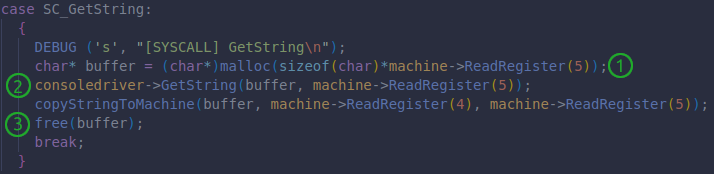
\includegraphics[width=\textwidth,height=\textheight,keepaspectratio]{Leak}
    \label{fig:fuites}
\end{figure}

\begin{figure}[h]
    \caption{Exécution du programme de test \textit{alloctypescomparison} avec allocation classique}
    \centering
    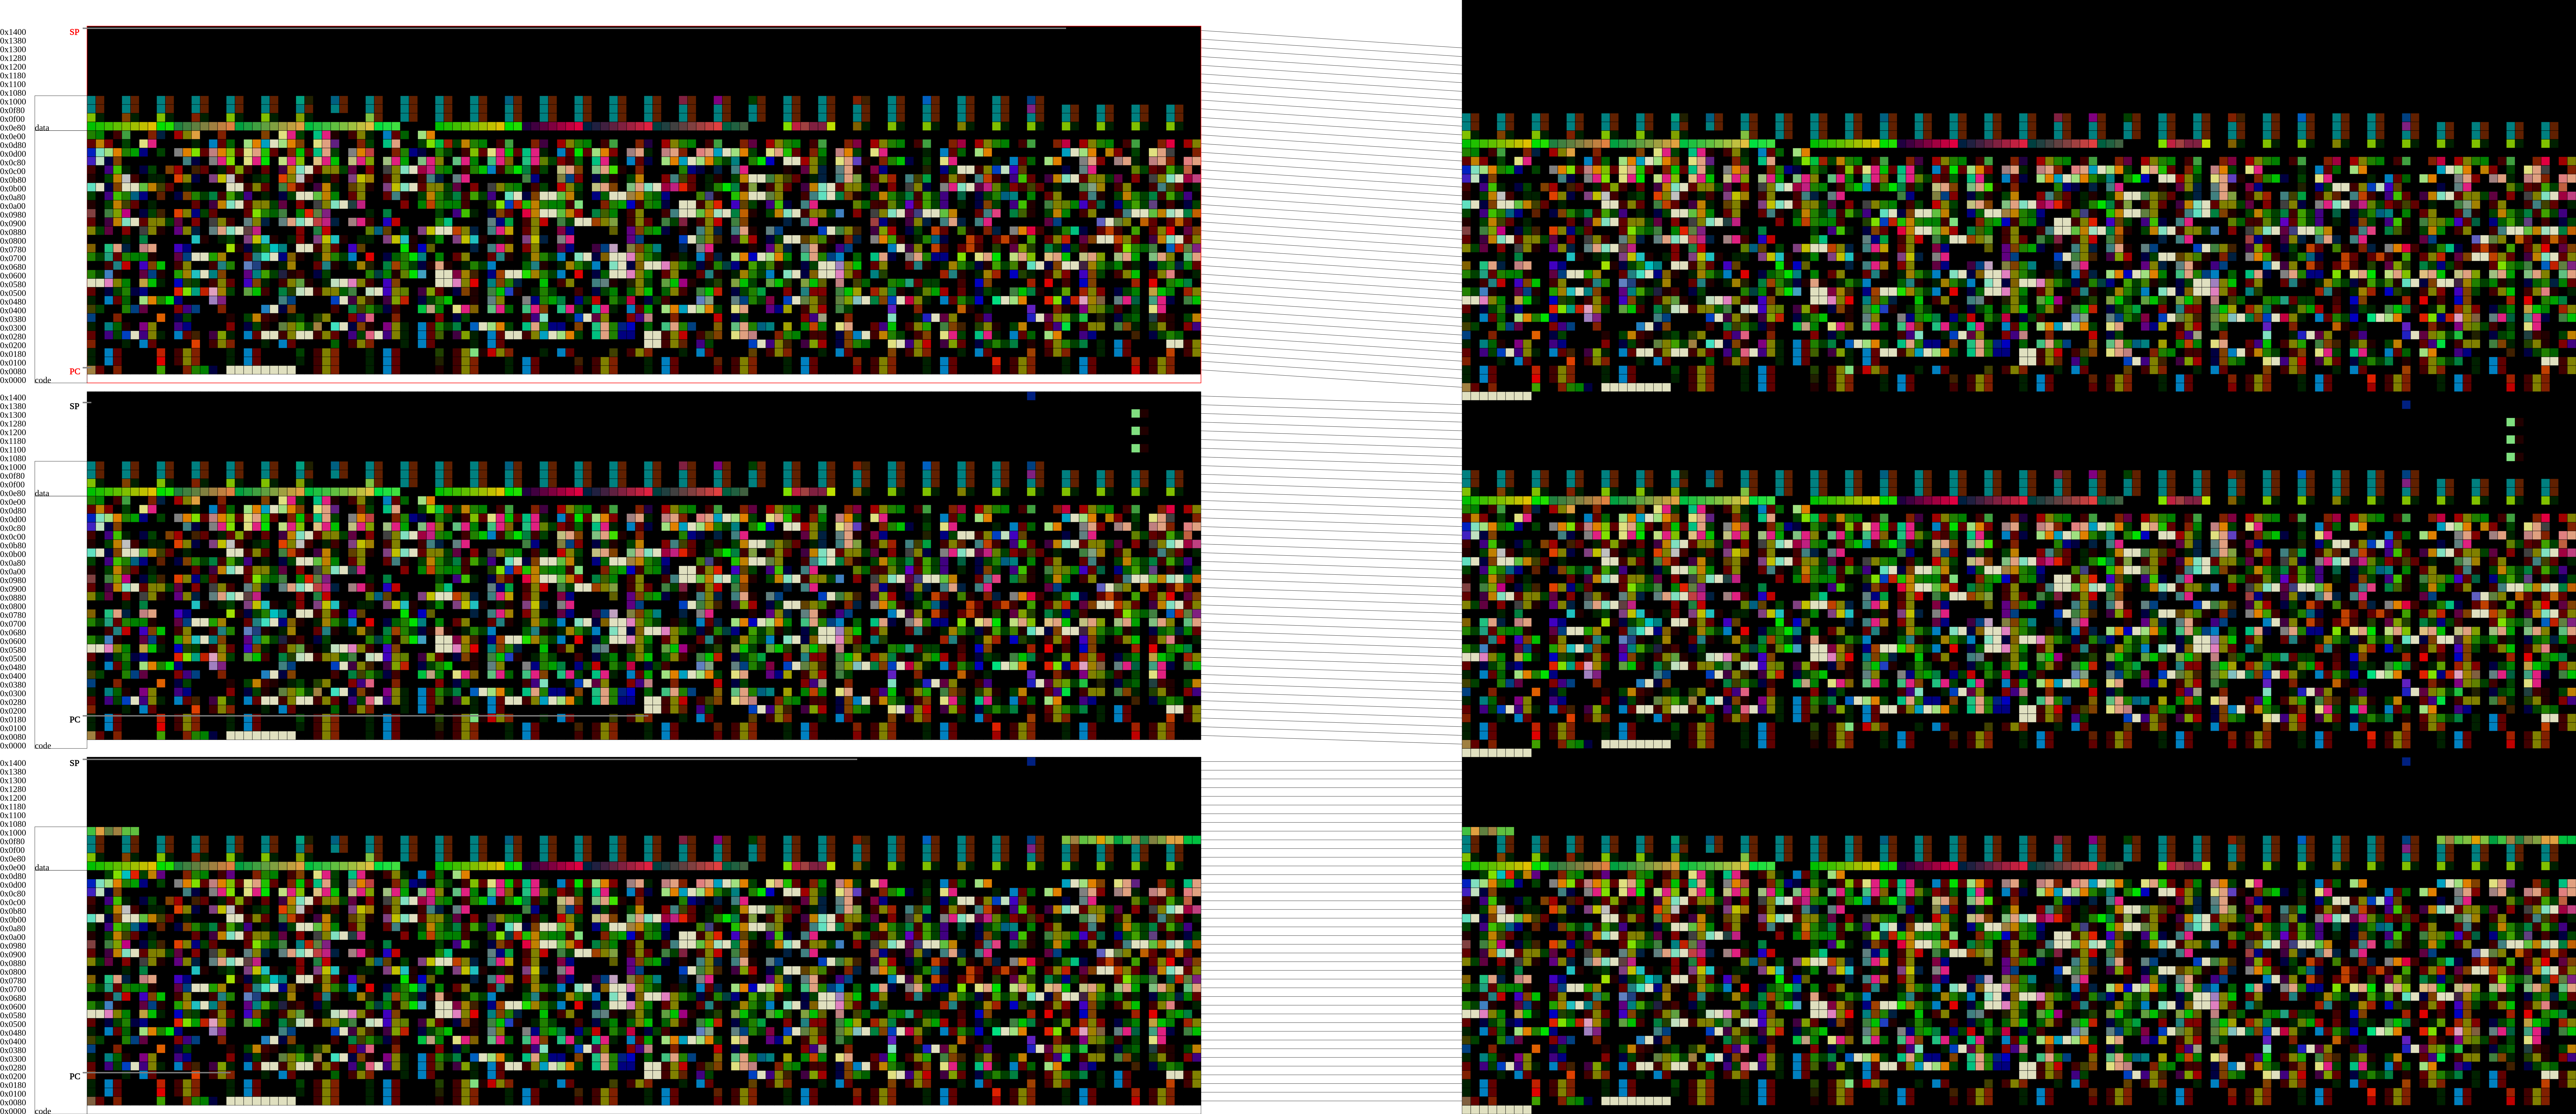
\includegraphics[width=\textwidth,height=\textheight,keepaspectratio]{memory_classic}
    \label{fig:alloc_classic}
\end{figure}

\begin{figure}[h]
    \caption{Exécution du programme de test \textit{alloctypescomparison} avec allocation aléatoire}
    \centering
    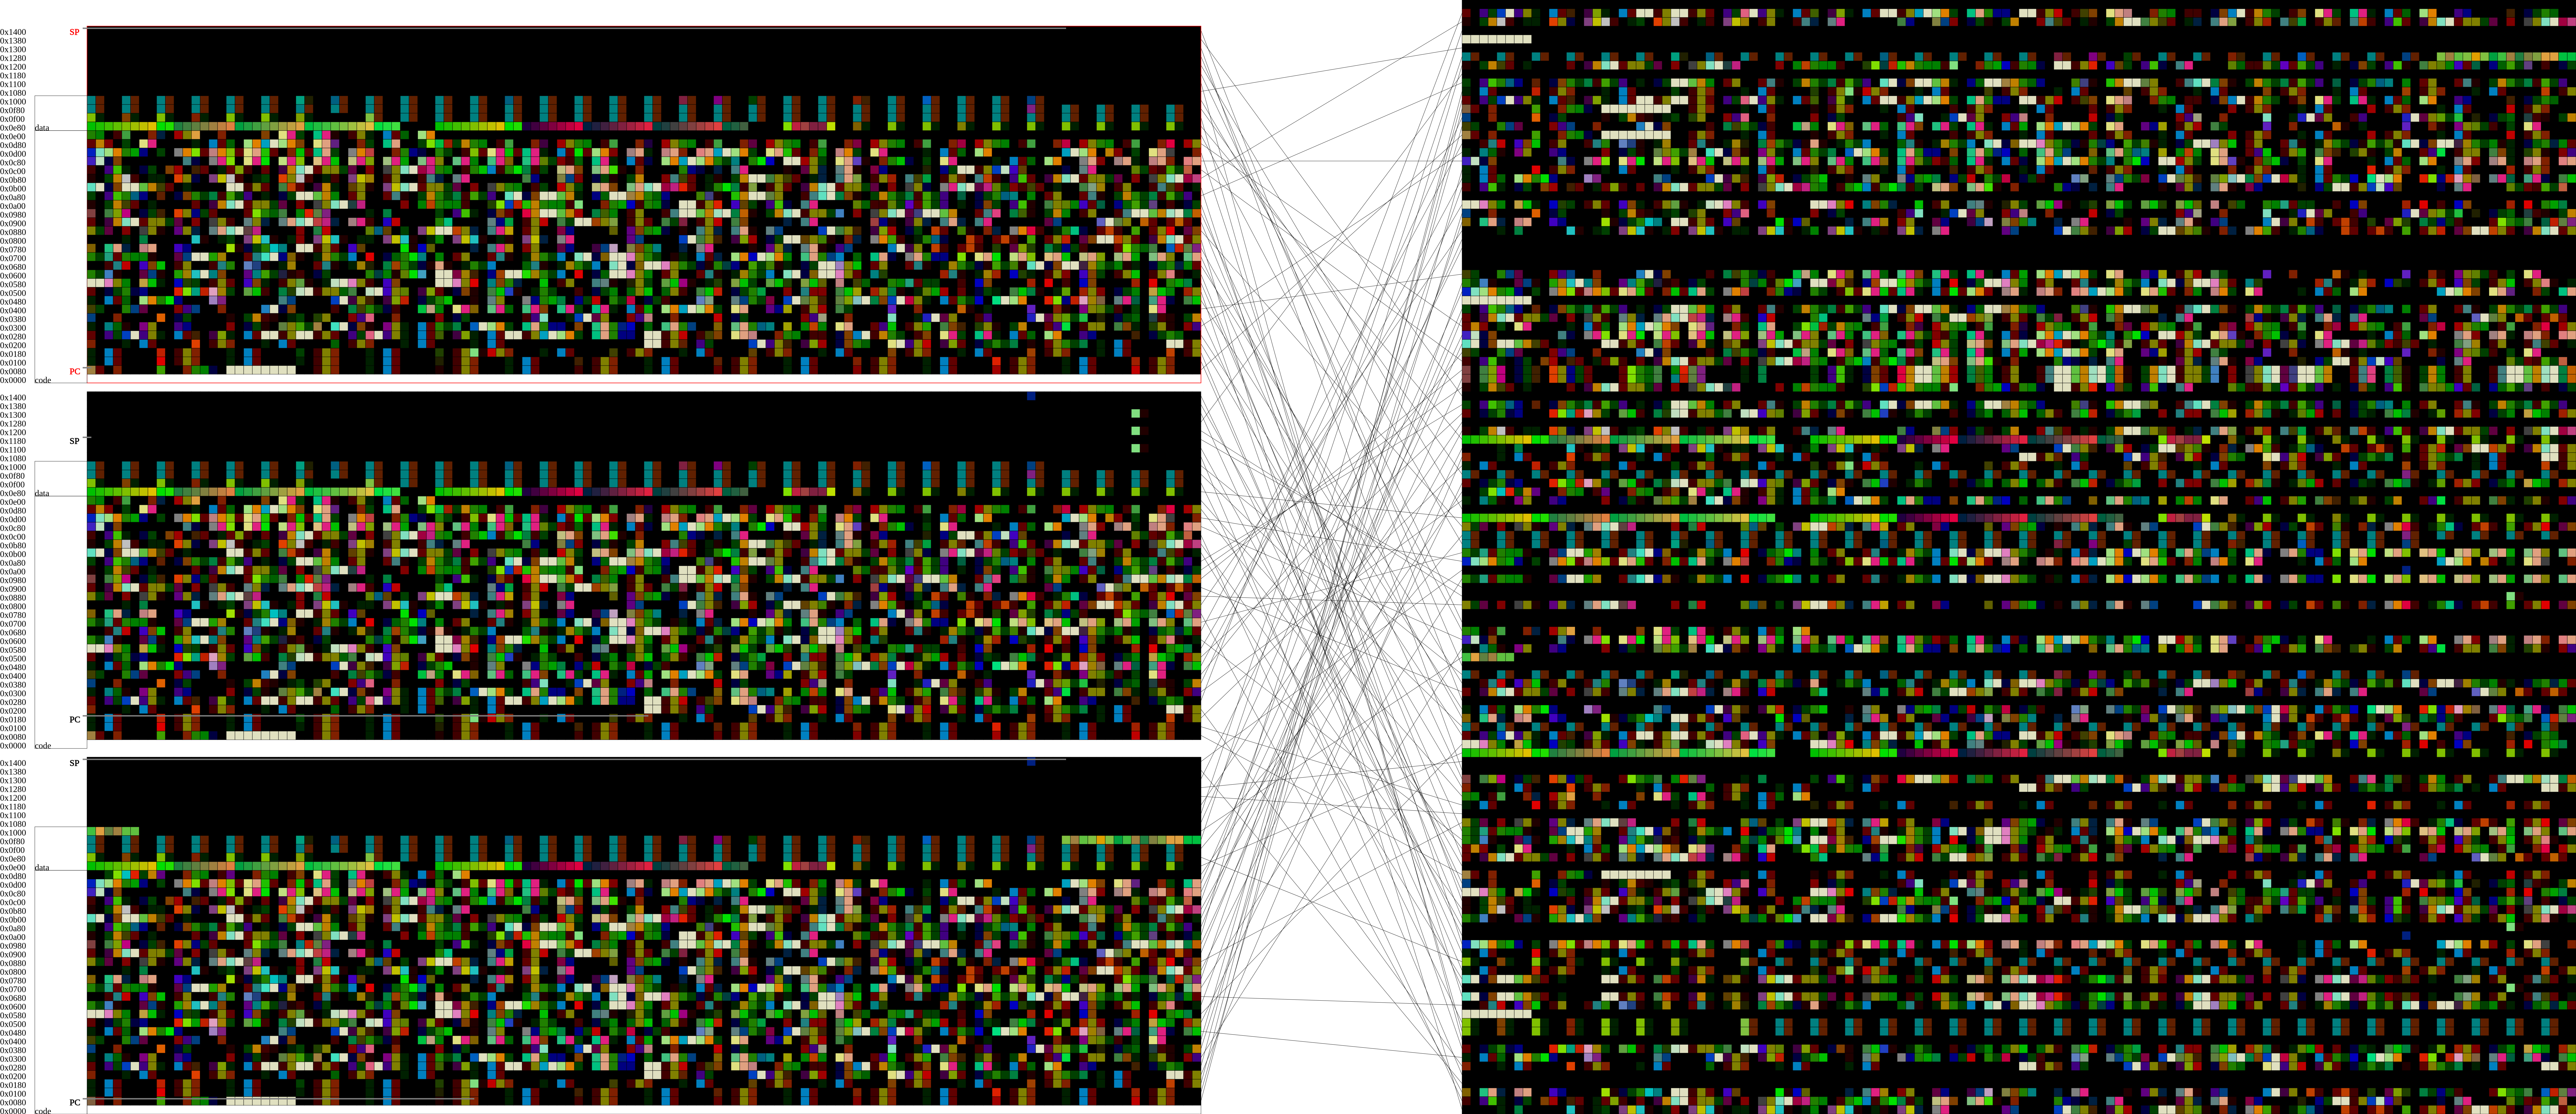
\includegraphics[width=\textwidth,height=\textheight,keepaspectratio]{memory_random}
    \label{fig:alloc_random}
\end{figure}

\end{document}